\chapter{Signal Chain%
  \label{chap:\currfilebase}}

  Some sensors operate at small energies. The signals are to weak to be converted into digital ones by standard components. \emph{Signal conditioning} enables us to amplify and denoise analog signals so that the signal can be further processed. In our application, both the load cell's and accelerometer's senors signal must be amplified to match the input range of their respective \ac{ADC}. In this section we put together all conditioning steps necessary from sensor to the digital signal under the term signal chain. Because the selected accelerometers come in \ac{IC} packages that include the complete signal chain, we focus on the signal chain of the load cell. For a quick introduction into signal conditioning and processing, read \secref{signal_conditioning_processing}. A schematic of a typical signal chain of an \ac{EMA} is shown in \figref{fig:measurement}.

\ac{LC}s that are based on strain gauges or piezoelectric ceramics both generate low-voltage respectively low-current signals when under stress. In strain gauge \ac{LC}s, it is the resistance that changes when it is stressed. Therefore, an electric energy supply is necessary to be able to generate a sensor signal. This makes the sensor an active one. With piezoceramics, it is possible to measure the current induced solely by the piezoelectric effect, which makes it passive; but especially in small sensors, preconditioning circuits are already integrated in the sensor so that one needs additional supply voltage for the conditioning and to get an amplified current or voltage signal. When looking at the voltage output signals, they vary in the range of a few \si{\milli\volt}. Standard components operate in the range of a few volts; therefore we need to amplify the signals first, if we want to use low-cost conditioning. The key components used to condition analog signals are filters. They are used to reduce the bandwidth to the range expected to be measured, cutting off unnecessary noise from outside this bandwidth. The last processing step in the analog signal chain is the conversion of the signal into a digital one, that is from a time-continuous, continuously valued signal into a discrete time-step and quantized one. This conversion presupposes the signal to be conditioned, so that the value range and frequency bandwidth are both limited to the maximum operation range of the \ac{ADC}, to meet the best possible resolution in time and amplitude of the signal in the digital realm. This can be achieved using at least one amplifier and one \ac{LPF}.

\section{Amplification}

The power of electrical signals is amplified by active electrical components that are configured to match different properties.
\begin{itemize}
  \item The \emph{gain} of an amplifier is a measure of the relative signal amplitude between output and input. Amplifiers with higher gains require smaller input signals for the same output amplitudes and are therefore more sensitive.
  \item The \emph{bandwidth} is the frequency range of satisfactory performance of an amplifier. Typically non-linear effects outside this region disturb the output signal.
  \item \emph{Efficiency} defines how much of the supply power can be converted into the output signal. Depending on the technology used, the efficiency may vary between 10~and~more~than~\SI{90}{\percent}. Note that lower efficiency amplifiers generate more heat during operation.
  \item \emph{Linearity} is a measure of how consistent the amplifier approaches a constant gain within its bandwidth. Typically, negative feedback loops are used to reduce non-linearities.
  \item \emph{Noise}, a side effect generated by all electronic components, is given by the noise factor, that is a comparison between the output signal noise and the thermal noise of the input signal.
  \item The \emph{output dynamic range} defines the ratio between the maximally allowed output signal power and the noise level of the system.
\end{itemize}

\subsection{Operational Amplifier}

Amplifiers apply signal gain on electrical inputs so that the output matches the input times a constant gain factor. The latter is determined by the impedance of the subsequent device in the signal chain and the magnitude at the input. But by setting the gain factor one predetermines the introduced absolute noise due to the amplifier's \ac{SNR}.

In simple amplifiers, the \ac{SNR} purely depends on the quality of the components and the environmental conditions. This can be bypassed by building differential setups, where amplifiers, like transistors and field transistors, are fed with both the non-inverted and the inverted input signal individually. With multi-staging and additional filter circuits one can reduce the noise further and ultimately the \ac{SNR} becomes strongly dependent on the circuit design and less dependent on the quality of each component. Specific to different applications, many variants of the described circuitry are available in so-called Operational Amplifiers (\acs{OPA}s).

\begin{figure}[htb!]
  \centering
  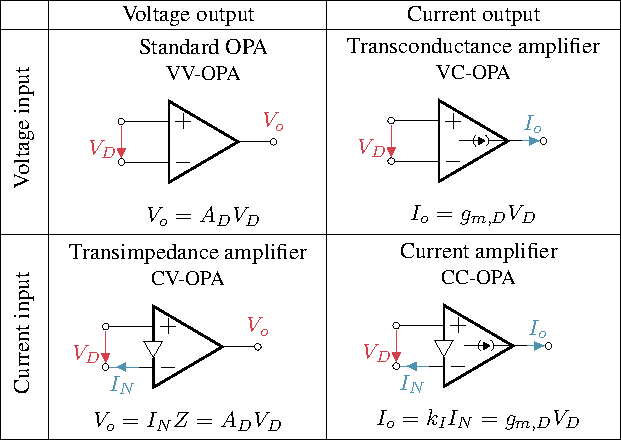
\includegraphics[scale=0.95]{figures/electronics/op_amp/op_amp_types/op_amp_types}
  \caption[Main OPA types]{Main operational amplifier types \cite{Tietze2008EC}%
  \label{fig:op_amp_types}}
\end{figure}

\ac{OPA}s are available in a variety of \ac{IC} packages and differ little from discrete transistors in terms of size and prize. In some packages even multiple individual \ac{OPA}s are included. Initially \ac{OPA}s offered high accuracy at low frequencies. Over time different circuit designs for different needs have broadened the field of application considerably. Today, it is hard to find a task that is better met by a transistor than by an \ac{OPA}. We subdivide the latter into four main types, as shown in \figref{fig:op_amp_types}. The differences are high-resistive or low-resistive inputs and outputs. The standard \ac{OPA} and the transconductance amplifier, for example, have high-resistance inputs. Therefore, they are voltage controlled. The outputs on the other hand are of low and high internal resistance respectively, where low-resistance outputs act as voltage sources and high-resistance outputs act as current sources. In the naming convention the two leading letters represent input and output. ``V'' at first position stands for a voltage controlled \ac{OPA} with a high-resistance input, where ``C'' means current controlled and low-resistive input. At the second position ``V'' and ``C'' define low- and high-resistance outputs that act as voltage and current source respectively.
The differential gain of an ideal VV-\ac{OPA} is given by the slope at the operating or bias point:
\begin{align}
  A_D &= \eval{\dv{V_o}{V_D}}_{b}
\end{align}
The transfer characteristics of an ideal \ac{OPA}s can be seen in \figref{fig:op_amp_transfer_cuves}. When dealing with current outputs the differential transconductance $g_{m,D}$ indicates the degree of output current increase with rising input voltage.
\begin{align}
  g_{m,D} &= \eval{\dv{I_o}{V_D}}_{b}
\end{align}

Although the major part of electronics is based on voltage controlled circuits, \ac{OPA} designs, different from the standard \ac{OPA} are preferable in some applications. Amplifiers with low-resistance inputs are better suited for high frequency applications. The main advantages of the latter are the lower oscillation tendency due to shortened internal signal paths and larger range of possible gains compared to high-resistance input \ac{OPA}s. When designing circuits with current amplifiers it is often easier to use the current transfer factor $k_I$ than the differential transconductance.
\begin{align}
  k_I &= \eval{\dv{I_o}{I_N}}_{b}
\end{align}

\begin{figure}[!htb]
  \sbox0{\subcaptionbox{Amplifier with voltage output\label{sfig:op_amp_transfer_volt}}{%
    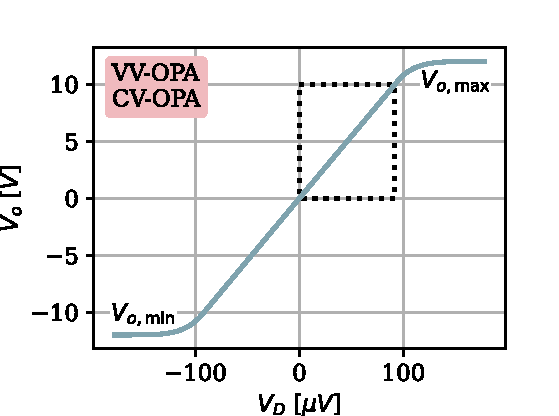
\includegraphics[scale=0.72]{figures/electronics/op_amp/op_amp_transfer_volt}
    }}% a
  \sbox1{\subcaptionbox{Amplifier with current output\label{sfig:op_amp_transfer_curr}}{%
    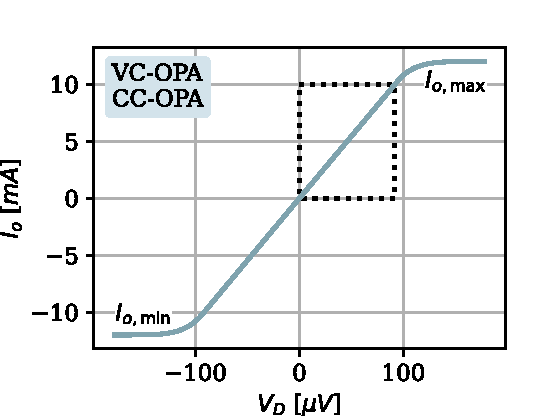
\includegraphics[scale=0.72]{figures/electronics/op_amp/op_amp_transfer_curr}
    }}% b
  \centering
  {%
    \renewcommand{\arraystretch}{6}%
    \setlength{\tabcolsep}{0em}
    \begin{tabular}{ccc}
      \usebox0 & \usebox1 \\
    \end{tabular}%
  }
  \caption[Transfer characteristics of OPAs]{Transfer characteristics of \ac{OPA}s, where the dotted square includes the line of positive operating or bias points.%
    \label{fig:op_amp_transfer_cuves}}
\end{figure}

Because of the differential circuit of the standard \ac{OPA}, it is normally powered by a symmetric voltage supply. But when working with digital circuits, one usually uses single power supplies. For these applications \ac{OPA}s were designed, that allow single supply voltage operation. Furthermore when one cannot use a higher voltage power supplies, rail-to-rail \ac{OPA}s will allow control of the signal output between the full range of the positive and negative supply voltage, allowing maximal amplification, see \figref{fig:opamp_controllability}.
When working with digital circuits, a single voltage supply is preferred. For this case one uses single supply voltage \ac{OPA}s. In this thesis \ac{OPA}s that were able to use both single and dual supply voltages were used.

\begin{figure}[!htb]
  \centering
  \subcaptionbox{Normal VV-\ac{OPA} compared to rail-to-rail VV-\ac{OPA} with supply voltages of $\pm\SI{5}{\volt}$}{%
    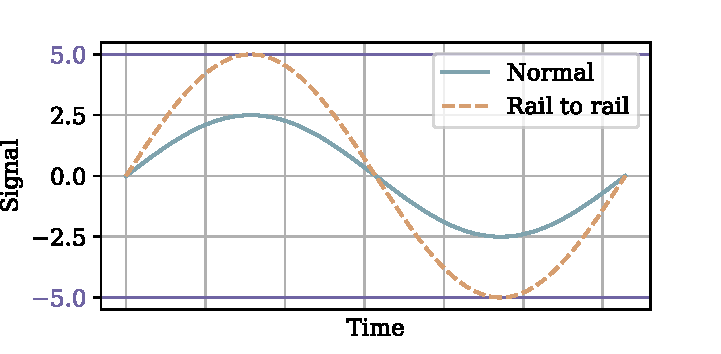
\includegraphics[scale=0.72]{figures/electronics/op_amp/plot_opamp_railrail}}
  \hspace{4em}
  \subcaptionbox{Single supply voltage VV-\ac{OPA} with a supply voltage of \SI{5}{\volt}}{%
    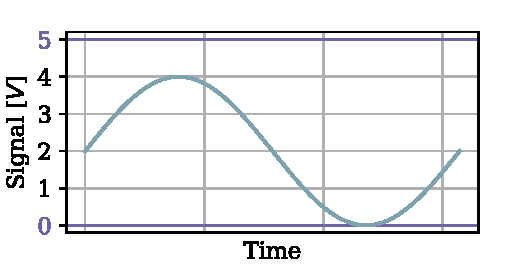
\includegraphics[scale=0.72]{figures/electronics/op_amp/plot_opamp_single}}
    \caption[Controllability of VV-\ac{OPA} signal outputs]{Controllability of VV-\ac{OPA} signal outputs%
    \label{fig:opamp_controllability}}
\end{figure}

\subsection{Mean Noise Figure and the Signal-to-Noise Ratio}
To determine the mean noise figure and the \acf{SNR} one needs conduct tests on an amplifier with a known signal. In its simplest form one can determine the \ac{SNR} and the mean noise figure by connecting a signal generator directly to the amplifier's input. In \cite{Tietze2008EC} \citeauthor{Tietze2008EC} write, that per definition, the \ac{SNR} is the ratio of the information containing signal power over the noise power:
\begin{align}
  \mathrm{SNR} &= \frac{P_{us}}{P_n}
\end{align}
where $P_n$ is the power in the application specific frequency interval $f_L<f<f_U$. We know that the power is proportional to the square of its effective value. The effective value, on the other hand, is defined as the root-mean-square of the electrical signal. Hence the noise of the signal generator is:
\begin{align}
  \mathrm{SNR}_g &= \frac{\nu_{g,\text{eff}}^2}{\nu_{r,\text{eff}}} = \frac{\nu_{g,\text{eff}}^2}{\displaystyle\int_{f_L}^{f_U} \abs{\vect{\nu}_{r,g}(f)}^2 \dd{f}} \label{eqn:snr_g}
\end{align}
An amplifier increases the noise density by the \emph{spectral noise figure} $F(f)$. The \ac{SNR} at the amplifier input is thus:
\begin{align}
  \mathrm{SNR}_i &= \frac{\nu_{g,\text{eff}}^2}{\nu_r} = \frac{\nu_{g,\text{eff}}^2}{\displaystyle\int_{f_L}^{f_U} \abs{\vect{\nu}_r(f)}^2 \dd{f}} = \frac{\nu_{g,\text{eff}}^2}{\displaystyle\int_{f_L}^{f_U} F(f)\abs{\vect{\nu}_{r,\text{eff}}(f)}^2 \dd{f}} \label{eqn:snr_i}
\end{align}
which is lower than the \ac{SNR} of the signal generator. Note that in a circuit, it is the comparison between the powers of the useful signal and the input noise, that determines the quality of the signal that is amplified. If the input signal is too low compared to the input signal noise, the noise contribution will dominate in the amplified signal.

The \emph{mean noise figure} corresponds to the relation of the \ac{SNR} ratios:
\begin{align}
  F &= \frac{\mathrm{SNR}_g}{\mathrm{SNR}_i} = \frac{\displaystyle \int_{f_L}^{f_U} F(f)\abs{\vect{\nu}_{r,g}(f)}^2 \dd{f}}{\displaystyle \int_{f_L}^{f_U} \abs{\vect{\nu}_{r,g}(f)}^2 \dd{f}} \label{eqn:mean_noise_figure}
\end{align}
And is usually quoted in decibels \si{\decibel}
\begin{align}
  F_{\si{\decibel}} &= 10\log F &F_{\si{\decibel}} &= \mathrm{SNR}_{g,\si{\decibel}} - \mathrm{SNR}_{g,\si{\decibel}}
\end{align}
When using an ideal signal generator, that has uniform noise density over all frequencies, \eqref{eqn:mean_noise_figure} simplifies to:
\begin{align}
  F &= \frac{1}{f_U-f_L}\int_{f_L}^{f_U} F(f)\dd{f}
\end{align}
Additionally, one can often assume the noise figure to be constant. Thus $F=F(f)$, which is generally referred to as the noise figure $F$.

In some applications the noise causes stronger interference in certain ranges of the given frequency interval than in other ranges. Then a weighted filter, whose absolute frequency response is proportional to the disturbing effect, is used to get more meaningful \ac{SNR}s. For this the noise density of the generator in the denominators of Equations~\ref{eqn:snr_g}~and~\ref{eqn:snr_i} are replaced by the \emph{weighted noise density}:
\begin{align}
  \abs{\vect{\nu}_{r(B),g}(f)}^2 &= \abs{\vec{H}_B(2\ju\pi f)}^2\abs{\vect{\nu}_{r,g}(f)}^2
\end{align}
with the transfer function of the weighted filter $\vect{H}_B(s)$.

Note that the bandwidth of the amplifier needs to cover at least the interval of the useful signal $f_L<f<f_U$ to provide equal amplification. Moreover, the bandwidth of the amplifier is usually wider than required, i.e.\ it amplifies the ranges $f<f_L$ and $f>f_U$ with operating gain $\vect{A}_B(s)$. It is in these ranges, where the signal only contains noise. Which means, that the amplifier, if not limited to the frequency range, provides the noise power at the output:
\begin{align}
  P_{n,o} &= \int_0^\infty \abs{\vect{A}_B(2\ju\pi f)}^2F(f)\abs{\vect{\nu}_{r,g}(f)}^2\dd{f} \label{eqn:p_no}
\end{align}
Considering that the signal is amplified by the useful gain $\vect{A}_{B,us}$, which is assumed to be constant over the useful range, the \ac{SNR} ath the amplifier output becomes:
\begin{align}
  \mathrm{SNR}_o &= \frac{\abs{\vect{A}_{B,us}}^2\nu_{g,\text{eff}}^2}{P_{n,o}} = \frac{\abs{\vect{A}_{B,us}}^2\nu_{g,\text{eff}}^2}{\int_0^\infty \abs{\vect{A}_B(2\ju\pi f)}^2F(f)\abs{\vect{\nu}_{r,g}(f)}^2\dd{f}}
\end{align}
Which is lower than $\mathrm{SNR}_i$, given by \eqref{eqn:snr_i}, since $P_{n,o}$ includes the total noise of all frequencies and not just the range $f_L<f<f_U$ used to define in $P_{n,i}$. Note that the components following the amplifier are primarily driven by the amplified noise, if the power at the output $P_{n,o}$ is considerably larger than the useful signal power. That said, the noise of the $P_{n,o}$ as defined in \eqref{eqn:p_no} is only of importance if the noise outside the useful range is transmitted. To reduce this signal component we apply a filter that reduces the bandwidth of the signal. Optimally this is a bandpass filter with lower and upper cutoff frequencies at $f_L$ and $f_U$.

If the noise densities of both the signal generator and the amplifier are almost constant in the transfer bandwidth, the noise power at the amplifier output can be approximated by:
\begin{align}
  P_{n,o} &\approx F\abs{\vect{\nu}_{r,g}}^2\int_0^\infty \abs{\vect{A}_B(2\ju\pi f)}^2\dd{f} = F\abs{\vect{\nu}_{r,g}}^2\abs{\vect{A}_{B,us}}^2 B_r
\end{align}
Where we defined the \emph{equivalent noise bandwidth} as:
\begin{align}
  B_r = \frac{\displaystyle\int_0^\infty \abs{\vect{A}_B(2\ju\pi f)}^2\dd{f}}{\abs{\vect{A}_{B,us}(2\ju\pi f)}^2}
\end{align}
This means that the area under the plot of the squared magnitude is replaced by the area of rectangle shown in \figref{fig:equivalent_noise_bandwidth}, i.e.\ the squared constant gain $\abs{\vect{A}_{B,us}}^2$ times the equivalent noise bandwidth $B_r$.

\begin{figure}[htb!]
  \centering
  \includegraphics[scale=1]{figures/electronics/op_amp/equivalent_noise_bandwidth}
  \caption[Equivalent Noise Bandwidth of an Amplifier]{Equivalent noise bandwidth of an amplifier \cite{Tietze2008EC}%
    \label{fig:equivalent_noise_bandwidth}}
\end{figure}

\newpage
\subsection{Instrumentation Amplifier}
In resistive sensor applications bridge circuits similar to \figref{sfig:wheatstone_bridge_single} are used. The two outputs of the bridge circuit each carry a signal that enables us to sense a change in resistance differentially. But because the circuit uses a constant supply voltage, a \emph{common-mode}, is present in both signals, i.e.\ a \ac{DC} voltage. If we use standard \ac{OPA}s for amplification, the differential signal is amplified, while the common-mode voltage receives unity gain. This is a common-mode reduction, the undesirable common-mode is still appearing in the output signal. In contrast, instrumentation amplifiers allow differential signal amplification and all common-mode rejection. It has got a two pin differential input and one single-ended output with respect to a reference terminal.

The \ac{CMR} is typically specified for the full range common-mode voltage change at a given frequency and source impedance:
\begin{align}
\mathrm{CMRR} &= \eval{\pqty{A_D(f=f_{\text{ref}})\frac{V_{\mathrm{CM}}}{V_{o}}}}_{Z_S} &\text{and}& &\mathrm{CMR} &= 20\cdot\log_{10}\mathrm{CMRR}
\end{align}
where
\begin{itemize}
  \item $A_D$ is the differential gain of the amplifier
  \item $V_{\mathrm{CM}}$ is the common-mode voltage present at the amplifier inputs
  \item $V_o$ is the output voltage, when the common-mode signal is applied
  \item $f_{\text{ref}}$ is the frequency at which the gain is measured
  \item $Z_S$ is the specified source impedance
\end{itemize}

\figref{fig:in_amp_circuit} shows the \ac{OPA} circuit of a typical instrumentation amplifier. The input buffer amplifiers pass the common-mode voltage through unity gain in both signals. The output signals of the two buffers then connect to the subtractor section where the differential signal is amplified and the common-mode voltage is attenuated. Note that the $R_G$ resistor is used to set the instrumentation gain, with higher resistance causing lower gains. For more background on instrumentation amplifiers, consult \cite{kitchin2006inst}.
Because
\begin{figure}[!htb]
  \centering
  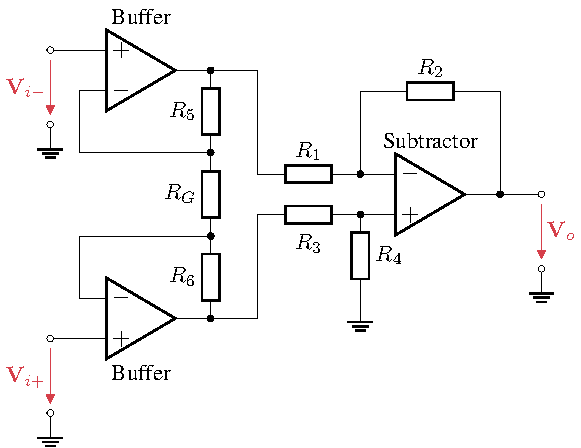
\includegraphics[scale=0.9]{figures/electronics/op_amp/in_amp_circuit/in_amp_circuit}
  \caption[Typical Instrumentation Amplifier Design]{Typical instrumentation amplifier design%
  \label{fig:in_amp_circuit}}
\end{figure}

\section{Filtering}
Whenever we measure a signal in the real world, it will inherently contain some form of noise. Filtering enables us to cut off contributions to the signal amplitude, that are outside the useful signal frequency bandwidth.

The two main types of filters are analog and digital ones, where the digital filters are more versatile, cost-effective and precise compared to their counterpart. Nevertheless, analog filters are required when dealing with analog signals, i.e.\ whenever the signal must be bandwidth limited. As described previously, it is advantageous if a signal is bandwidth limited before it is amplified, because we do not want to amplify the noise components of the signal. Furthermore electric devices in the signal chain may be bandwidth limited as well; disturbances of the signal occur due to frequency dependent phase shifts or damping when operating outside these ranges. Namely when digitizing a signal, the additional effect of aliasing may disturb a signal significantly if it contains frequency components above the Nyquist frequency.

We operate at a low frequencies in the frame of this thesis. The useful bandwidth of the lower modes in \ac{EMA} of \ac{MT}s range typically between a few ten and a few hundred hertz. Therefore, we focus on a lowpass-filter design, so that there is no miss on the lowest eigenfrequencies. For simplicity, from this point on onward the term bandwidth addresses the upper bandwidth limit, while the lower limit remains near zero. Additionally, the cutoff frequency refers to the lowpass cutoff frequency. For more details on other filter designs we recommend the textbooks for analog electronics and filter design \cite{Tietze2008EC, Stiny2019AeB} and \cite{williams2014analog}. The content in this Section is reliant on the theories found in these books.

\subsection{Passive Lowpass Filters}
The frequency response of the simplest \ac{LPF}, as shown in \figref{fig:lp_passive_1ord}, can be expressed as
\begin{align}
  \vect{H}(\ju\omega) &= \frac{\vect{v}_o}{\vect{v}_i} = \frac{1}{1+\ju\omega RC}
\end{align}
By replacing $\ju\omega$ by $\ju\omega+\sigma = s$ one can express the transfer function as
\begin{align}
  H(s) &= \frac{\LT{V_o(t)}}{\LT{V_i(t)}} = \frac{1}{1 + sRC}
\end{align}

\begin{figure}[htb!]
  \centering
  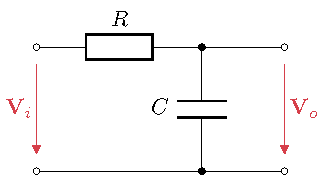
\includegraphics[scale=1]{figures/electronics/lowpass/lp_passive_1ord/lp_passive_1ord}
  \caption[Passive first-order \ac{LPF}]{Simplest passive \ac{LPF} of first-order%
    \label{fig:lp_passive_1ord}}
\end{figure}

This is the ratio between the Laplace transformed time-domain signals of the output and input respectively. We then generalize the result by normalizing the complex frequency variable $s$ by defining
\begin{align}
  s_n &= \frac{s}{\omega_c}
\end{align}

For further simplification one can set $\sigma$ to zero; which is equivalent to assuming sinusoidal form of the input signal.
Thus, for $\sigma=0$
\begin{align}
  s_n &= \frac{\ju\omega}{\omega_c} = \ju\frac{f}{f_c} = \ju\omega_n
\end{align}

The cutoff frequency of the circuit in \figref{fig:lp_passive_1ord} is $f_c=1/(2\pi RC)$. By definition the normalized complex frequency variable thus becomes $s_n=2\pi RC$. Therefore, the transfer function can be written as
\begin{align}
  H(s_n) &= \frac{1}{1+s_n}
\end{align}

The magnitude $\abs{\vect{H}(\ju\omega_n)}$ and phase $\varphi=\angle\vect{H}(\ju\omega_n)$ of the transfer function for sinusoidal signals are then given by
\begin{align}
  \abs{\vect{H}(\ju\omega_n)}^2 &= \frac{1}{1+\omega_n^2} &&\text{and} &\varphi &= \angle\vect{H}(\ju\omega_n) = \arctan\frac{1}{1 + \ju\omega_n}
\end{align}

For frequencies $\omega_n\gg 1$ one can approximate $\abs{\vect{H}}=1/\omega_n$. This corresponds to a reduction in gain of \SI{20}{\decibel} per frequency decade.

If a sharper cutoff is required, $N$ \ac{LPF}s can be connected in series. The \ac{TF} then becomes
\begin{align}
  \vect{H}(s_n) &= \prod\limits_{i=1}^{N}\frac{1}{1+\alpha_i s_n}
\end{align}
where $\alpha_i$ are real and positive coefficients and for frequencies $\omega_n\gg 1$, $\abs{\vect{H}}\approx 1/\omega_n^N\propto 1/\omega^N$. The gain therefore falls off at $N\cdot\SI{20}{\decibel}\:\text{per decade}$. It can be observed that the \ac{TF} posesses $N$ real and negative poles. This is characteristic of $N$th-order passive $RC$ \ac{LPF}.

If we cascade \ac{LPF}s with identical cutoff frequencies, then
\begin{align}
  \alpha &= \alpha_i = \sqrt{\sqrt[N]{2}-1}
\end{align}
which is the condition for which \emph{critical damping} occurs. Each individual cutoff frequency is a factor $1/\alpha$ higher than that of the filter as a whole.

The \ac{TF} of the $N$th-order \ac{LPF} has the general form
\begin{align}
  H(s_n) &= H_0 \pqty{1 + \sum\limits_{i=1}^N c_i s_n}^{-1} \label{eqn:lpf_nthord_tf_general}
\end{align}
where $c_i$ are real and positive coefficients and the order of the filter is equal to the highest power of $s_n$. By rewriting the denominator in factored form and allowing complex poles, one denotes \autoref{eqn:lpf_nthord_tf_general} as
\begin{align}
  H(s_n) &= \frac{H_0}{(1+a_1s_n+b_1s_n^2)(1+a_2s_n+b_2s_n^2)\cdots} \label{eqn:lpf_nthord_tf_poles}
\end{align}
where $a_i$ and $b_i$ are real and positive coefficients and $b_1=0$ for odd orders $N$.

The frequency response can be optimized to different theoretical aspects by setting the coefficients $a_i$ and $b_i$. As a consequence of these optimizations, complex poles arise, that cannot be realized by blocks of passive $RC$ filters. It is possible to meet the optimized conditions by using $LRC$ filters with the simplest example shown in \figref{fig:lp_passive_2ord}, where
\begin{align}
  &&H(s) &= \frac{1/(LC)}{s^2+\frac{R}{L}s+\frac{1}{LC}} &&\text{and} &f_c &= \frac{1}{2\pi\sqrt{LC}}&&
\end{align}
This design does not pose any difficulties when opting for high cutoff frequencies. But it is apparent, that one requires the use of large capacitances as well as large inductances for low cutoff frequencies. And because large inductances are unwieldy and have poor electrical properties, an active filter design is better suited for low cutoff frequencies. With these designs the use of inductances are avoided by the addition of active elements, namely \ac{OPA}s, to the $RC$ network.

\begin{figure}[htb!]
  \centering
  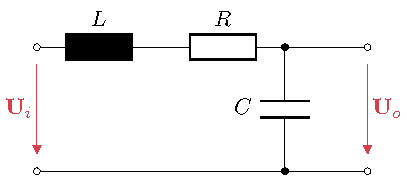
\includegraphics[scale=1]{figures/electronics/lowpass/lp_passive_2ord/lp_passive_2ord}
  \caption[Passive second-order \ac{LPF}]{Passive second-order \ac{LPF}, $LRC$ circuit%
    \label{fig:lp_passive_2ord}}
\end{figure}

\newpage
\subsection{Optimizations of Lowpass Filters}
Following \citeauthor{Tietze2008EC}~\cite{Tietze2008EC}, we take the \emph{standard form} of the second-order \ac{LPF} into consideration, where:
\begin{align}
  H(s_n) &= \frac{H_0}{1+a_1s_n+b_1s_n^2} = \frac{k}{\displaystyle 1+\frac{s_n}{Q}+s_n^2} = \frac{k}{1+2\zeta s_n+s_n^2} \\
  Q &= \frac{1}{2\zeta} = \frac{b_1}{a_1}
\end{align}
where $k$ is the gain factor and $Q$ is the quality factor repsectively $\zeta$ the damping ratio. In the case of unity gain, $k=1$, one can see that the two poles are given by:
\begin{align}
  p_{1,2} &= (-\zeta \pm \sqrt{\zeta^2-1})\omega_n
\end{align}
and that the poles are\dots
\begin{itemize}
  \item real if $\zeta\geq 1$
  \item complex if $0<\zeta<1$
  \item imaginary if $\zeta=0$
  \item in the right half plane and unstable with $\mathrm{Re}\Bqty{p}>0$ if $\zeta<0$
\end{itemize}
If we now take a look at the second-order system used to describe the accelerometer dynamics in \eqref{eqn:acceler_dynamics} and replace the static sensitivity $K$ with the gain factor $k$ the system dynamics are equal and one can see the influence of the damping factor on the system behavior in \figref{fig:seismic_accelerometer_edited}.
Many filter designs expose this configurability of a second order systems. Because of parameters $k$ and $\zeta$ respectively $Q$ to tune the filter behavior and gain different optimization points targeted. Moreover, when connecting multiple second-order filters in series to realize higher-order filters with steeper roll-offs, the individual second-order filter parameters can be tuned to match three distinct optimization points:

\begin{itemize}
  \item The \emph{Chebyshev} filter is optimized to have a steep roll-off rate but shows ripple in the pass- and stopband.
  \item The \emph{Butterworth} filter is optimized to have the most stable gain at the passband but has a poor roll-off rate.
  \item The \emph{Bessel} filter is optimized to have the most stable phase response, which is critical for fast signal level changes. The caveat comes in form of the poorest roll-off of all filters, when compared at same order.
\end{itemize}

The influence of the order on the filter gain can be seen in \figref{fig:lp_filter_mag}. Above, the passband refers to frequency contributions below the cutoff frequency and the stopband is defined depending on the application. If one expects high noise densities directly above the cutoff frequency, the stop band needs to be defined at a low gain and the roll-off of the filter must be designed to be steep, whereas if some application only allows small phase shifts, the latter cannot be achieved by a high order filter. The definition of the cutoff frequency is more consistent. For most filters the cut-off frequency is reached, when the gain falls short by \SI{3}{\decibel}, i.e\ when when the filter halves the squared gain, which in turn is proportional to the power transmission. An exception is the Chebyshev filter. Here it is common to define the cutoff the point where the filter roll-off reaches minus the maximally allowed ripple gain in decibel, see \figref{fig:lp_lowpass_pass_stopband}.
Note that given the three optima, any hybrid filter design between the Chebyshev and the Butterworth as well as between the Butterworth and Bessel is possible too.

\begin{figure}[!htb]
  \centering
  \subcaptionbox{Standard normalization, cutoff frequency at \SI{-3}{\decibel}\label{sfig:lp_filter_2ord_bessel_bp}}[0.45\textwidth]{%
    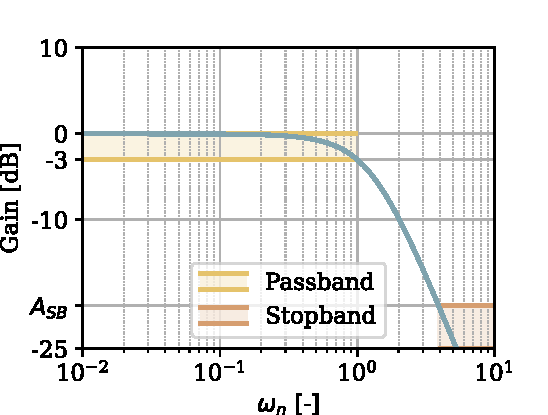
\includegraphics[scale=0.72]{figures/electronics/lowpass/lp_filter_2ord_bessel_bp}}
  \hfill
  \subcaptionbox{Chebyshev normalization, cutoff frequency at negative the allowed ripple $A_{\max}/A_{\min}$\label{sfig:lp_filter_2ord_cheby_bp}}[0.45\textwidth]{%
    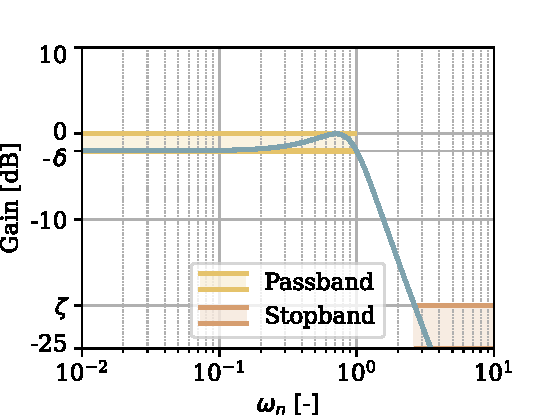
\includegraphics[scale=0.72]{figures/electronics/lowpass/lp_filter_2ord_cheby_bp}}
  \caption[\ac{LPF} Pass- and Stopband]{\ac{LPF} Pass- and Stopband, where the passband is defined by $\omega_n<1$ and the stopband is chosen depending on the application (usually starting at \SIrange{-20}{-160}{\decibel})%
    \label{fig:lp_lowpass_pass_stopband}}
\end{figure}

When comparing the step and impulse responses in \figref{fig:lp_filter_4ord_step} and \figref{fig:lp_filter_4ord_imp}, it becomes apparent that one must trade better frequency-cutoff with worse signal response in the time domain. This is because the change in phase over the frequency, i.e.\ the group delay, is almost constant in the Bessel filter, whereas the Chebyshev optimization, tuned to maximum gain roll-off speed, induces fast changes in the phase. This causes the undesired swinging in the time signals. This The phase responses can be compared in \figref{fig:lp_filter_pha}. A more in depth look at the group delay is given in the following description of the Bessel filter.

\begin{figure}[!htb]
  \centering
  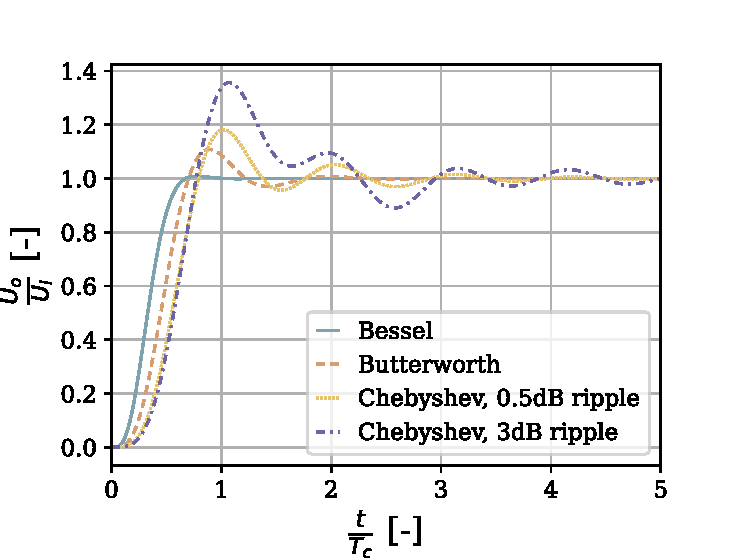
\includegraphics[scale=0.68]{figures/electronics/lowpass/lp_filter_4ord_step}
  \caption[Step response of fourth-order \ac{LPF}]{Step response of fourth-order \ac{LPF} --- Note, that the Chebyshev filter is represented with the cutoff frequency at \SI{-3}{\decibel} for comparability.%
    \label{fig:lp_filter_4ord_step}}
\end{figure}

Until now we described all-pole \ac{LPF}s, i.e.\ no nodes are present in the filter system, as can be seen in the \ac{TF} \eqref{eqn:lpf_nthord_tf_poles}. With filter designs that include nodes, one can realize sharper cutoffs without increasing the phase shift. Generally more complex filter curves are possible at the cost of more unstable behavior and more complex filter design. Due to these disadvantages their behavior is not as reliable as the filters listed before. Therefore they were not considered during this thesis. For more background on these filters, also called \emph{elliptic-function} filters, we advice to take look at the textbook \cite{williams2014analog}.

\begin{figure}[!htb]
  \centering
  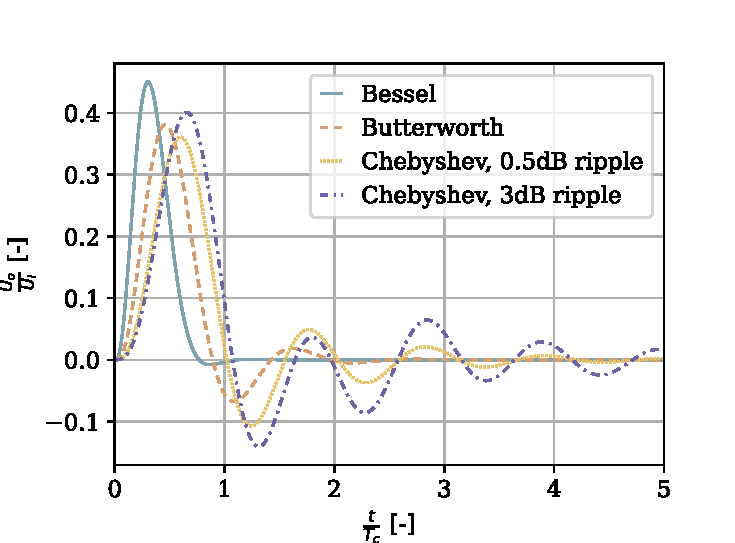
\includegraphics[scale=0.68]{figures/electronics/lowpass/lp_filter_4ord_imp}
  \caption[Impulse response of fourth-order \ac{LPF}]{Impulse response of fourth-order \ac{LPF} --- Note, that the Chebyshev filter is represented with the cutoff frequency at \SI{-3}{\decibel} for comparability.%
    \label{fig:lp_filter_4ord_imp}}
\end{figure}

\subsubsection{Butterworth Lowpass Filter}
From the general solution in \autoref{eqn:lpf_nthord_tf_general} the squared absolute gain in \ac{LPF}s takes the form
\begin{align}
  \abs{\vect{H}(\omega_n)}^2 &= H_0^2 \pqty{1 + \sum\limits_{i=1}^N k_{2i}\omega_n^{2i}}^{-1}
\end{align}
where odd powers of $\omega_n$ do not occur, since $\abs{\vect{H}}^2$ must be an even function. In Butterworth \ac{LPF}s the function $\abs{\vect{H}}^2$ must be maximally flat at $\omega_n < 1$, i.e.\ for frequencies below the cutoff frequency. This condition is best met if we only keep the highest order term, since lower order terms contribute the most to the denominator at low frequencies, decreasing the gain. Hence, for Butterworth \ac{LPF}s
\begin{align}
  \abs{\vect{H}(\omega_n)}^2 &= \frac{H_0^2}{1+k_{2N}\omega_n^{2N}} \label{eqn:butterwoth_gain_squared}
\end{align}
where $k_{2N}=1$ due to the normalizing condition, which states that the square of the gain is reduced by \SI{3}{\decibel} at $\omega_n=1$, i.e. $\abs{\vect{H}(\omega_n=1)}^2 = \abs{\vect{H}(\omega_n=0)}^2/2$.

When implementing a Butterworth \ac{LPF}, one needs to consider the complex gain $\vect{H}$ involved in \autoref{eqn:butterwoth_gain_squared}. It can be determined by solving for coefficients $c_i$ in \autoref{eqn:lpf_nthord_tf_general}, given the squared gain of \autoref{eqn:butterwoth_gain_squared}. It is then possible to solve the transfer function analytically by combining complex conjugate poles. In the solution, we obtain the coefficients $a_i$ and $b_i$ of the quadratic expression in \autoref{eqn:lpf_nthord_tf_poles}
\begin{align*}
  \intertext{even order $N$:}
  a_i &= 2\cos\frac{(2i-1)\pi}{2N} &\text{for}\: &i = 1,2,\dots.\frac{N}{2}\\
  b_i &= 1
  \intertext{odd order $N$:}
  a_2 &= 1,\qquad a_i =2\cos\frac{(i-1)\pi}{N} &\text{for}\: & i=2,3,\dots,\frac{N+1}{2}\\
  b_1 &= 0,\qquad b_i =1
\end{align*}

\afterpage{%
\begin{figure}[!htb]
  \centering
  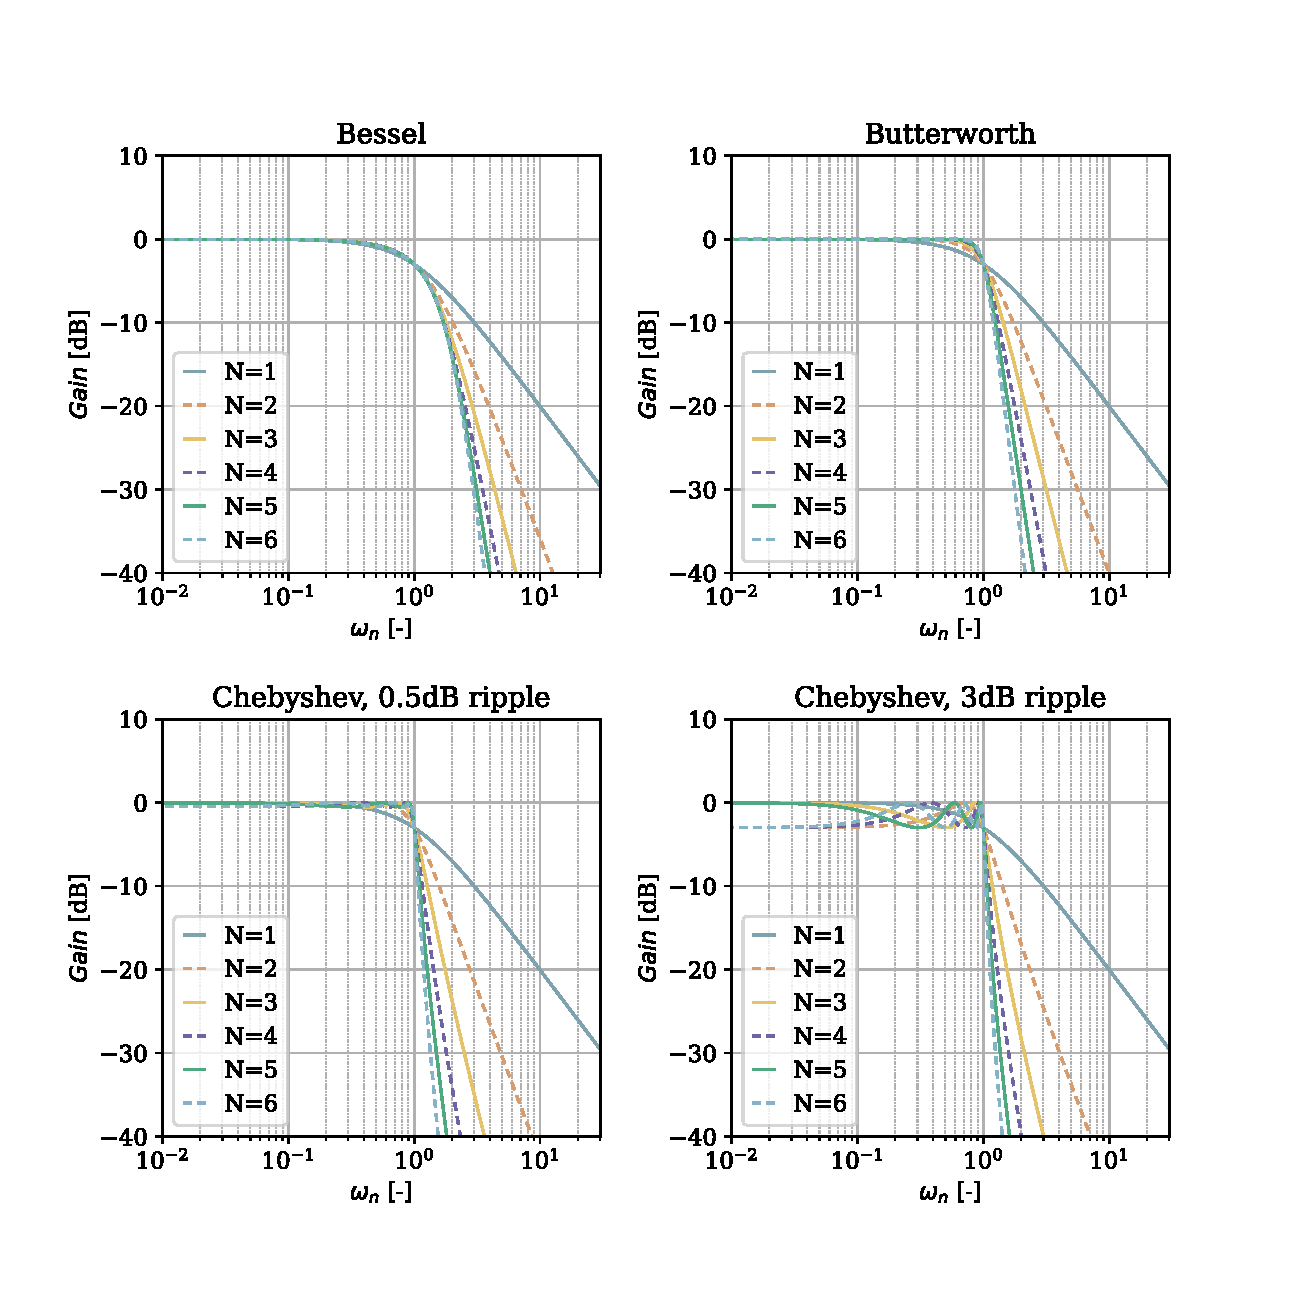
\includegraphics[scale=0.68]{figures/electronics/lowpass/lp_filter_mag}
  \caption[Influence of \ac{LPF} order $N$ on the amplitude of the frequency response]{Influence of \ac{LPF} order $N$ on the amplitude of the frequency response --- Note, that the Chebyshev filter is represented with the cutoff frequency at \SI{-3}{\decibel} for comparability.%
    \label{fig:lp_filter_mag}}
\end{figure}
\clearpage
}

\subsubsection{Chebyshev Lowpass Filter}
In the passband the Chebyshev \ac{LPF} is allowed to have a predetermined ripple. The characteristic of Chebyshev polynomials is, that the ripple ripples are constant, i.e.\ their local extrema in the gain plot can be connected by two horizontal lines that are displaced by the predetermined ripple.
\begin{align}
  T_N(x) &=\left\{%
    \begin{aligned}
      &\cos(N \arccos x),  &\text{for}\;&0\leq x\leq 1\\
      &\cos(N \arccosh x), &\text{for}\;&x>1
    \end{aligned}
  \right.
\end{align}
To get the \ac{LPF} frome these Chebyshev polynomials, we define
\begin{align}
  \abs{\vect{A}}^2 &= \frac{kA_0^2}{1+\varepsilon^2T_N^2(x)}
\end{align}
where $A_0$ is the so called DC- or zero-gain and the constant $k$ is chosen such that, for $x=0$, the square of the gain $\abs{\vec{A}}^2$ becomes $A_0^2$. If $N$ is even, this means $k=1$ and if $N$ is odd, we set $k=1+\varepsilon^2$; where the latter is a measure of the ripple and is given by
\begin{align}
  &\frac{A_{\max}}{A_{\min}} = \sqrt{1+\varepsilon^2}\\
  \intertext{and}
  &\left.\begin{aligned}
    A_{\max} &= A_0\sqrt{1+\varepsilon^2}\;\\
    A_{\min} &= A_0
  \end{aligned}\right\}
  \quad\text{if}\;N\;\text{is even}
  &&\left.\begin{aligned}
    A_{\max} &= A_0\\
    A_{\min} &= A_0/\sqrt{1+\varepsilon'2}\;
  \end{aligned}\right\}
  \quad\text{if}\;N\;\text{is odd}
\end{align}
Once $\abs{\vect{A}}^2$ is determined, the complex gains can be calculated. However, it is easier to derive the poles of the transfer function directly of the Butterworth filters. By combining the complex conjugates the coefficients $a_i$ and $b_i$ in \eqref{eqn:lpf_nthord_tf_poles} are determined:
\begin{align*}
  \left.\begin{aligned}
    b_i' &= \frac{1}{\cosh^2\gamma - \cos^2\frac{(2i-1)\pi}{2N}}\;\\
    a_i' &= 2b_i'\cdot\sinh\gamma\cdot\cos\frac{(2i-1)\pi}{2N}
  \end{aligned}\right\}&
  \quad\begin{aligned}
    &\text{if}\;N\;\text{is even and}\\
    &\text{for}\;i=1\dots\frac{N}{2}
  \end{aligned}\\
  \left.\begin{aligned}
    b_1' &= 0\\
    a_1' &= 1/\sin\gamma\\
    b_i' &= \frac{1}{\cosh^2\gamma - \cos^2\frac{(i-1)\pi}{N}}\;\\
    a_i' &= 2b_i'\cdot\sinh\gamma\cdot\cos\frac{(i-1)\pi}{N}
  \end{aligned}\right\}&
  \quad\begin{aligned}
    &\text{if}\;N\;\text{is odd and}\\
    &\text{for}\;i=2\dots\frac{N+1}{2}
  \end{aligned}\\
  \text{where}\; \gamma = &\frac{1}{N}\arcsinh\frac{1}{\varepsilon}
\end{align*}

The obtained coefficients $a_i'$ and $b_i'$ define a Chebyshev filter at the cutoff frequency $\omega_x$, which the gain assumes the value $A_{\min}$ for the last time. For easy comparison with other filter types we want to evaluate the filter at a cutoff frequency where the gain is \SI{-3}{\decibel}. For this we multiply the normalized frequency $s_n$ with a real constant $\alpha$, changing the quadratic expressions in the denominator of \eqref{eqn:lpf_nthord_tf_poles} to
\begin{align*}
  (1 + a_i'\alpha s_n + b_i'\alpha^2s_n^2)
\end{align*}
Next, we evaluate $\alpha$, so that the gain value is $1/\sqrt{2}\estimates\SI{-3}{\decibel}$ at the normalized frequency $s_n=\ju$. The coefficients for the filter with cutoff frequency pass through at \SI{-3}{\decibel} can then be determined by multiplication with the constant.
\begin{align}
  &&a_i &= \alpha a_i' &\text{and}& &b_i &= \alpha^2b_i'&& \label{eqn:broken_denominator}
\end{align}

{%
\begin{figure}[!htb]
  \centering
  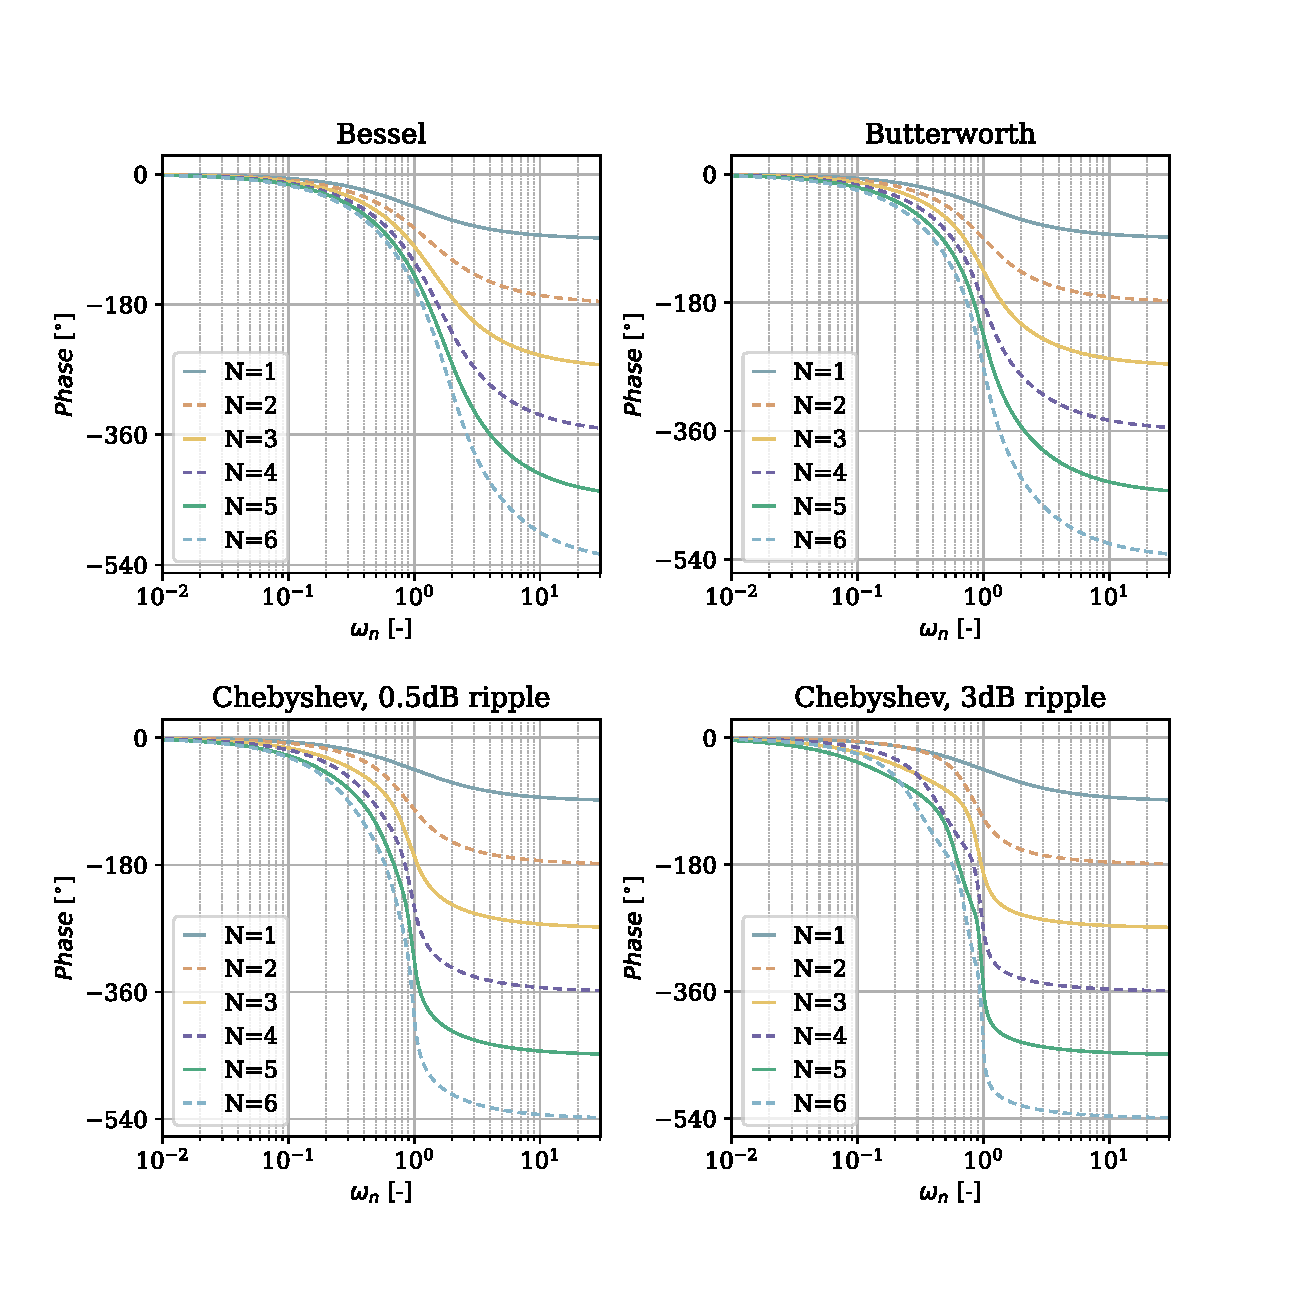
\includegraphics[scale=0.68]{figures/electronics/lowpass/lp_filter_pha}
  \caption[Influence of the \ac{LPF} order $N$ on the  phase of the frequency response]{Influence of the \ac{LPF} order $N$ on the  phase of the frequency response --- Note, that the Chebyshev filter is represented with the cutoff frequency at \SI{-3}{\decibel} for comparability.%
    \label{fig:lp_filter_pha}}
\end{figure}
\clearpage
}

\subsubsection{Bessel Lowpass Filter}
In the step and impulse response, \figref{fig:lp_filter_4ord_step}~and~\ref{fig:lp_filter_4ord_imp}, the Butterworth and Chebyshev filters show considerable overshoot. With the Bessel or also called Thomson filter we aim to mitigate this effect in order to create smooth response curves. It can be shown, that best square-wave responses are obtained when the \emph{group delay} of the filter is constant with respect to the frequency. The condition for the lowpass Bessel filter therefore sets the group delay in the passband maximally flat. The group delay $t_{gr}$ is defined as the negative of the change in phase shift due to frequency change.
\begin{align}
  t_{gr} &= -\dv{\varphi}{\omega}
\end{align}
Often we use the normalized group delay for calculations
\begin{align}
  T_{gr} &= t_{gr}\omega_c = 2\pi t_{gr}f_c = 2\pi\frac{t_{gr}}{T_c}
\end{align}
And given that the reciprocal of the cutoff frequency is by definition $T_c=2\pi/\omega_c$
\begin{align}
  T_{gr} &= -\omega_c\dv{\varphi}{\omega} = -\dv{\varphi}{\omega_n}
\end{align}

As an example, we consider the gain of a second-order \ac{LPF} given by~\eqref{eqn:lpf_nthord_tf_poles} and assume sinusoidal signals, i.e.\ $s=\ju\omega$. The phase shift of this system is
\begin{align}
  \varphi &= -\arctan\frac{a_1\omega_n}{1-b_1\omega_n^2}
\end{align}

Thus by calculating the negative of the derivative with respect to the normalized frequency, we get the normalized group delay
\begin{align}
  T_{gr} &= \frac{a_1(1+b_1\omega_n^2)}{1+(a_1^2-2b_1)\omega_n^2+b_1^2\omega_n^4}
\end{align}
For small frequencies, where $\omega_n\ll 1$, we can neglect the fourth order terms and this simplifies to
\begin{align}
  T_{gr} &= a_1\frac{1+b_1\omega_n^2}{1+(a_1^2-2b_1)\omega_n^2}
\end{align}
Now $T_{gr}=f(\omega_n^2)$ and we can find the coefficient configurations where it becomes independent of $\omega_n^2$, that is
\begin{align}
  &&b_1 &= a_1^2-2b_1 &\text{or}& &b_1 &= \frac{1}{3}a_1^2&&
\end{align}
A second equation to determine the coefficients is given, when we set the gain at the cutoff frequency to \SI{-3}{\decibel}, i.e.\ $\abs{A}^2=1/2$ at $\omega_n=1$.
\begin{align}
  \frac{1}{2} &= \frac{1}{(1-b_1)^2+a_1^2}
\end{align}

The calculations of higher order filters become more involved, since a system of nonlinear equations arises. But using a different approach one can find a recursion formula for the coefficients in \eqref{eqn:lpf_nthord_tf_general}.
\begin{align}
  &&c_1' &= 1 &\text{and}&  &c_i' &= \frac{2(N-i+1)}{i(2N-i+1)}c_{i-1}'\quad\text{for}\;i=2\dots N&&
\end{align}

But note, that this approach gives the coefficient for \SI{3}{\decibel} frequency cutoffs at $\omega_n=0$. To find the coefficients at for a usable cutoff frequency, we apply the same approach as we did with the Chebyshev coefficients. For that we rewrite the equation in form of \eqref{eqn:lpf_nthord_tf_poles} to get the second-order filter coefficients $a_i'$ and $b_i'$, apply the transformation $s_n=\alpha\ju\omega_n$ and solve for $\alpha$. The coefficients $a_i$ and $b_i$ can then be calculated with \eqref{eqn:broken_denominator}.

{%
\begin{figure}[!htb]
  \centering
  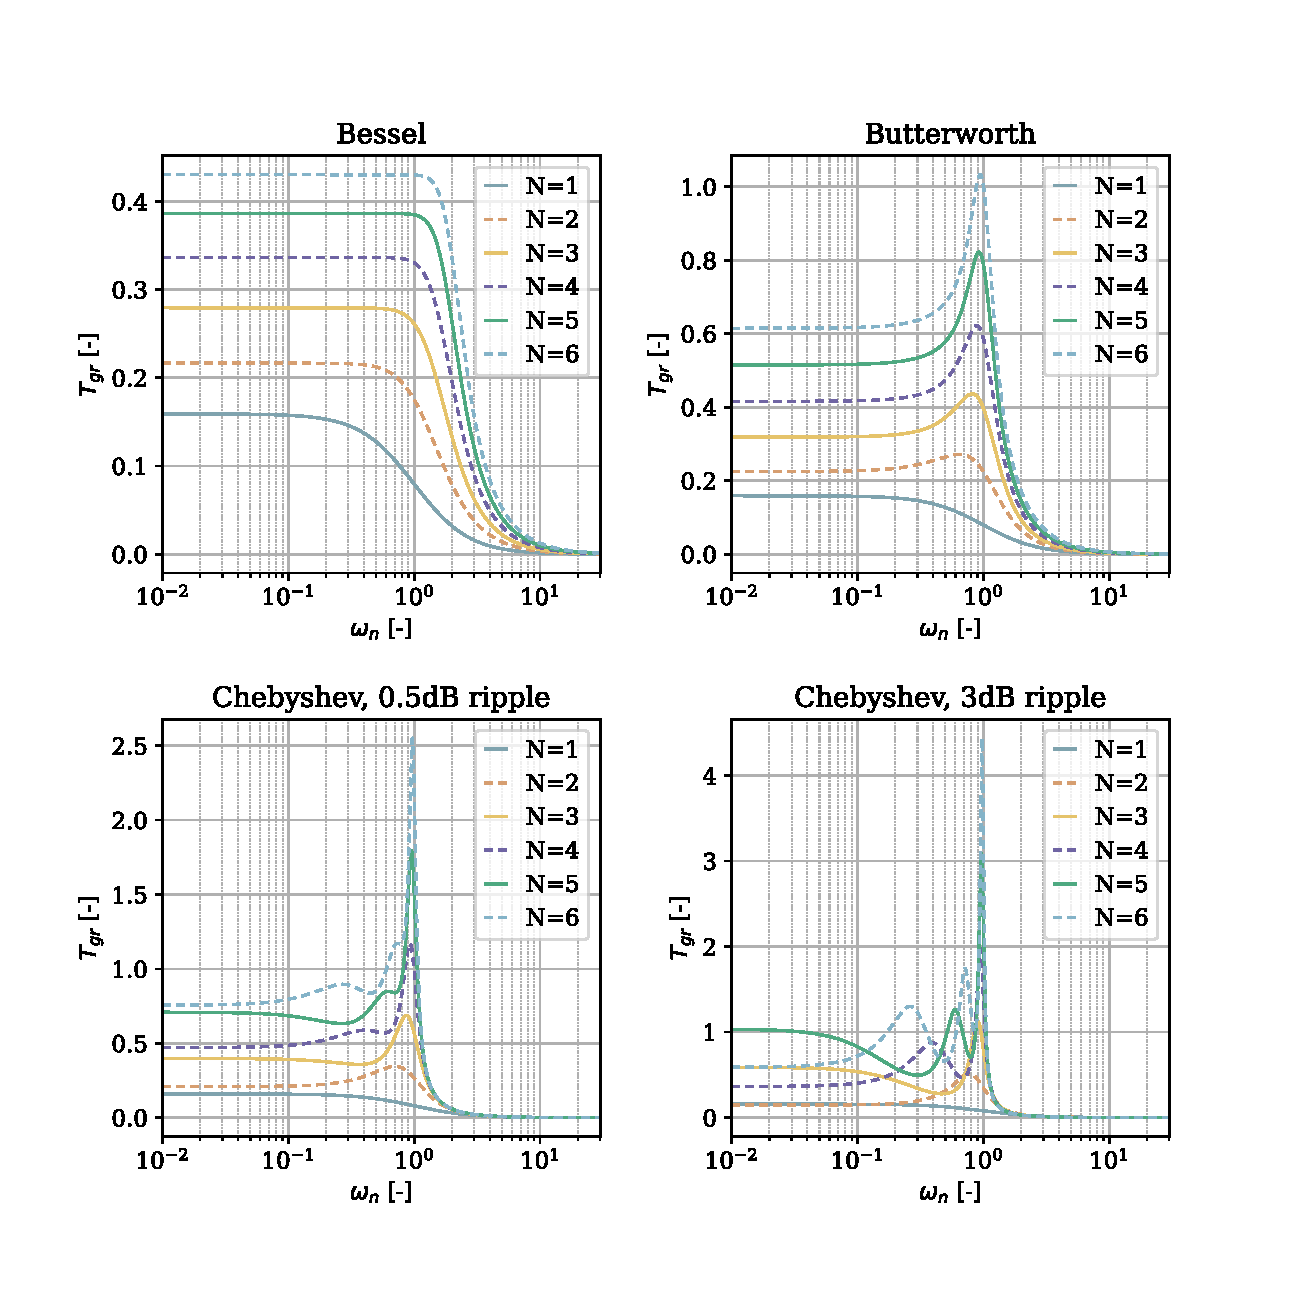
\includegraphics[scale=0.68]{figures/electronics/lowpass/lp_filter_grd}
  \caption[Influence of the \ac{LPF} order $N$ on the group delay of the frequency response]{Influence of the \ac{LPF} order $N$ on the group delay of the frequency response --- Note, that the Chebyshev filter is represented with the cutoff frequency at \SI{-3}{\decibel} for comparability.%
  \label{fig:lp_filter_grd}}
\end{figure}
\clearpage
}

\subsection{Active Filter Topologies}
Depending on the desired filter optimization target, one can choose the best suited topology to approach its \ac{TF}. First-order topologies are the noninverting and the inverting \ac{LPF}, see \figref{fig:lp_active_1ord_top}. Note that the negative sign in the \ac{TF} of the inverting amplifier generates a \SI{180}{\degree} phase shift from input and output. Furhtermore, at unity gain both $R_1$ and $R_2$ tolerances have an influence on the gain; therefore the noninverting impedance \ac{LPF} is preferred if one is looking for high unity gain accuracy.

\begin{figure}[!htb]
  \centering
  \subcaptionbox{Active first-order \ac{LPF} with impedance converter\label{sfig:lp_active_1ord_imp_conv}}
    {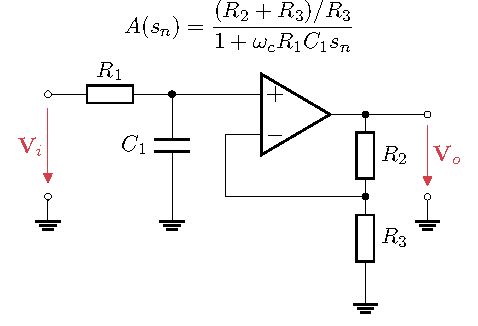
\includegraphics[scale=0.95]{figures/electronics/lowpass/lp_active_1ord_imp_conv/lp_active_1ord_imp_conv}}
    \hspace{4em}
  \subcaptionbox{Active first-order \ac{LPF} with inverting amplifier\label{sfig:lp_active_1ord_inv_amp}}
    {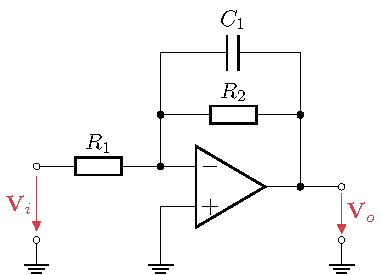
\includegraphics[scale=0.95]{figures/electronics/lowpass/lp_active_1ord_inv_amp/lp_active_1ord_inv_amp}}
  \\[0.5em]
  \caption[First-Order Lowpass Filter Topologies]{First-order lowpass filter topologies%
    \label{fig:lp_active_1ord_top}}
\end{figure}

The Sallen-Key topology is a common building block for filters. It is best used for applications that do not require sharp cutoffs. Since it is difficult to generate large Q-factors with this design.
\begin{figure}[!htb]
  \centering
  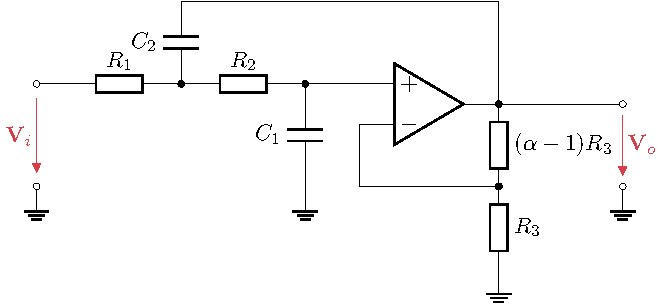
\includegraphics[scale=0.95]{figures/electronics/lowpass/lp_active_2ord_pos/lp_active_2ord_pos}
  \caption[Active Second-Order \ac{LPF} With Single Positive Feedback]{Active second-order \ac{LPF} with single positive feedback, Sallen-Key%
    \label{fig:lp_active_2ord_pos}}
\end{figure}

%\begin{figure}[!htb]
%  \centering
%  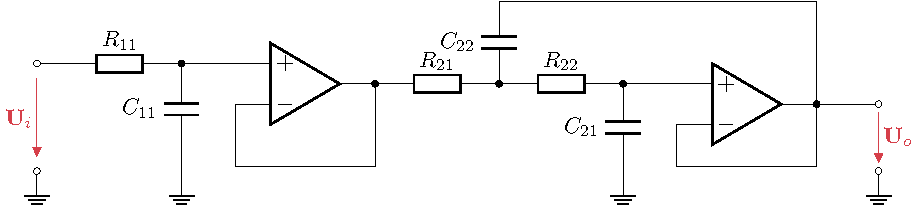
\includegraphics[scale=0.95]{figures/electronics/lowpass/lp_active_3ord_bessel/lp_active_3ord_bessel}
%  \caption[Active third-order \ac{LPF}]{Active third-order \ac{LPF}%
%    \label{fig:lp_active_3ord_bessel}}
%\end{figure}
%
%\begin{figure}[!htb]
%  \centering
%  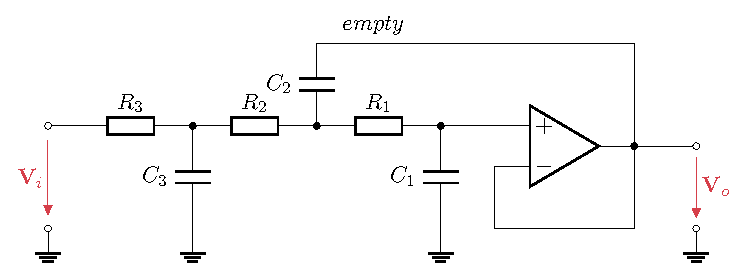
\includegraphics[scale=0.95]{figures/electronics/lowpass/lp_active_3ord_bessel_simple/lp_active_3ord_bessel_simple}
%  \caption[Simplified active third-order \ac{LPF}]{Simplified active third-order \ac{LPF}%
%    \label{fig:lp_active_3ord_bessel_simple}}
%\end{figure}

\newpage
\subsection{Anti Aliasing Filter}
The \acf{AAF} is used ahead of \ac{ADC}s to reduce the signal bandwidth. More precisely, it aims to reduce the aliasing effect, i.e.\ the artificial distortion of signals, that occurs when sampling at a finite frequency. The effect that aliasing can have on a signal is visualized in \figref{fig:plot_aliasing}. Here two analog sinusoidal signals are sampled at the same sampling frequency $f_s$. The digitized signal will always be a approximation of the analog one, but it is clear that the signal with $f<f_{\max}$ has a better approximation in its digital form, and most importantly, it is an approximation of same frequency in contrast to the signal with $f>f_{\max}$.

\begin{figure}[!htb]
  \centering
  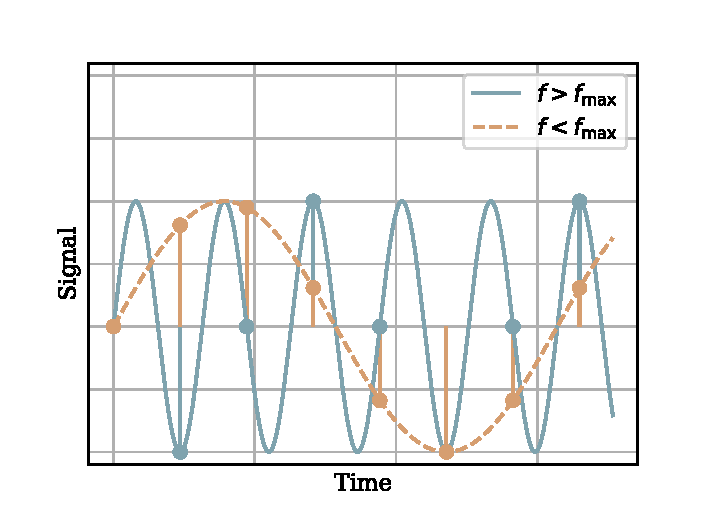
\includegraphics[scale=0.72]{figures/electronics/aaf/plot_aliasing}
  \caption[Aliasing]{Aliasing effect --- Note, that two analog sinusoidal signals of different frequencies are shown and sampled at the same frequency $f_s$. Interpolating the discrete points gives the respective digital signals, where the signal with frequency $f<f_{\max}$ gives a good approximation of its analog form and the signal with frequency $f>f_f{\max}$ connects to a lower frequency signal in its digital form.%
    \label{fig:plot_aliasing}}
\end{figure}

More specifically, when we take the \acf{FT} of the signal with $f>f_{\max}$ we see a peak of the absolute amplitude at a new frequency $f_d\leq f_s<f$. Similarly, when using input signals with multiple frequency components, the signal gain distorted by components in from the domain $f>f_{\max}$. This distortion is the result of overlapping signal components, which makes them indistinguishable. This is called aliasing.

For signals that are bandwidth limited, i.e\ their \ac{FT} is zero outside a finite region, the \emph{Nyquist-Shannon} sampling theorem finds that if those signals are sampled at $f_s=2f_{\max}$, where $f_{\max}$ is the highest frequency component, it is completely determined. Therefore, we want to cut off all frequency components above $f_s/2$ before digitizing any signal.
\clearpage

\section{Analog to Digital Conversion}

The \ac{ADC} shows internal noise that can be categorized into two uncorrelated main sources. The quantization noise and the thermal noise. The total internal noise can thus be expressed as the Euclidean norm of these two sources.

\begin{align}
  N_\text{ADC} &= \sqrt{N_{\text{ADC},\text{Thermal}}^2 + N_{\text{ADC},\text{Quantization}}^2}
\end{align}

Quantization noise is present due to the process of mapping an infinite number of possible electrical signal values in an analog signal to a finite number of digital codes. Subsequently, any digital output corresponds to an infinite number of analog inputs within range of the output value, plus and minus half the \ac{LSB} size, $s_\text{LBS}$. One can decrease quantization noise by choosing a higher resolution \ac{ADC}.

\begin{align}
  s_\text{LBS} &= \frac{V_{FSR}}{2^m}
\end{align}
where
\begin{itemize}
  \item $V_{\text{FSR}}$ is the full-scale range of the analog input value and
  \item $m$ is the resolution in number of bits
\end{itemize}

\begin{figure}[!htb]
  \centering
  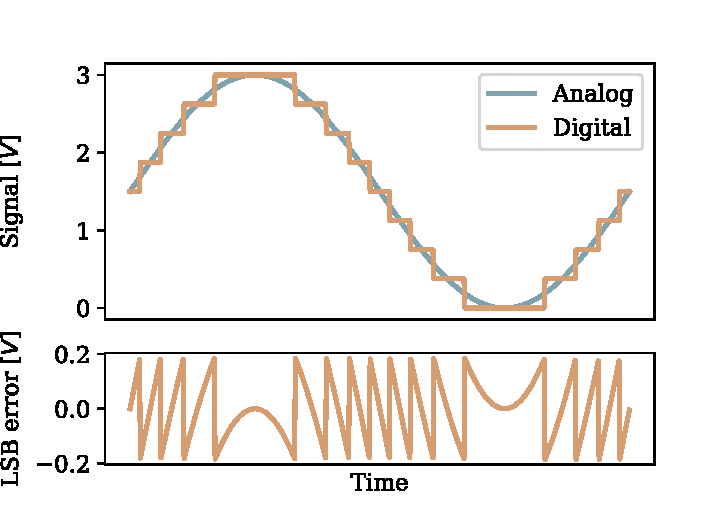
\includegraphics[scale=0.72]{figures/electronics/adc/plot_lsberr}
  \caption[ADC LSB waveform]{\ac{ADC} --- Analog input, digital output and \ac{LSB} error waveform with $s_\text{LBS} = \SI{375}{\milli\volt}$\cite{hall2020fund}%
    \label{fig:plot_lsberr}}
\end{figure}

Thermal noise is a phenomenon inherent in all electrical components. Because of this, it is a function of the device design and cannot be affected by the embedded system designer. Typically, one assumes the thermal noise to have a Gaussian distribution.

\begin{figure}
  \centering
  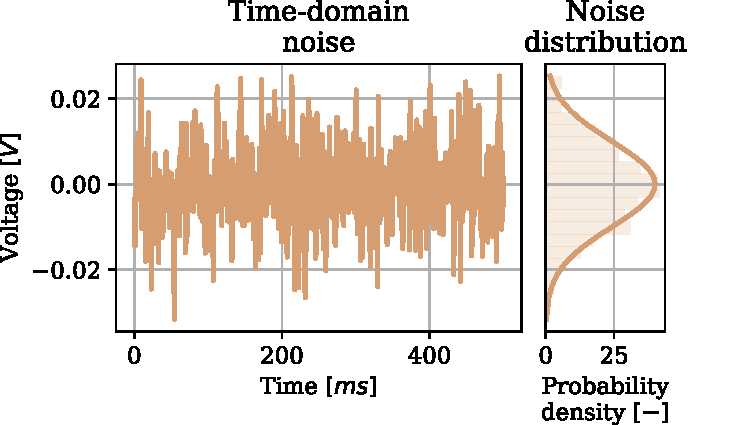
\includegraphics[scale=0.72]{figures/electronics/adc/plot_thermerr}
  \caption[ADC thermal noise]{ADC --- Thermal noise in the time domain with Gaussian probability density~\cite{hall2020fund}%
    \label{fig:plot_themerr}}
\end{figure}

Depending on the relative noise contributions of each source, we divide \ac{ADC}s into two extremes. Low- and high resolution \ac{ADC}s. Characteristic for a low-resolution \ac{ADC} is that $N_{\text{ADC},\text{Quantization}}\gg N_{\text{ADC},\text{Thermal}}$. Here the quantization noise dominates because of the large \ac{LSB} size. Typcally, starting above \SI{16}{\bit} resolution we decimates the \ac{LSB} so that the thermal noise becomes dominant. Within the low-cost system operate primarily with low-resolution \ac{ADC}s.

\subsection{Topologies}
\ac{SAR} \ac{ADC}s have a low-power consumption and are available in very small packages. This makes them them the preferred option for mobile devices as well as general purpose applications and data acquisition systems. An additional advantage of the \ac{SAR} topology is the negligible or zero latency. Its power consumption is proportional to the sampling rate.

The delta-sigma \ac{ADC}s offer the highest-resolution and are generally preferred in precision applications. Because they are highly integrated, they replace many components of a data acquisition system. In this topology a digital filter is included, typically optimized for the application. Its disadvantages are medium power consumption and cycle latency.

\begin{table}
  \centering
  {\renewcommand{\arraystretch}{1}%
  \footnotesize
  \begin{tabular}{lccp{4cm}}
    \toprule
    \multicolumn{1}{c}{\acs{ADC} Topology} & \makecell{Data rates\\/ \si{\mega S\per\second}} & \multicolumn{1}{c}{\makecell{Resolution\\/ \si{\bit}}} & \makecell{Benefits}\\
    \midrule
    \acs{SAR} & $\leq 4$ & $\leq 18$ & \vspace*{-1\baselineskip}%
      \begin{itemize}%
        \item simple implementation
        \item no latency
        \item low power
      \end{itemize}\\
    delta-sigma & $\leq 10$ & $\leq 28$ & \vspace*{-1\baselineskip}%
      \begin{itemize}%
        \item high resolution
        \item high integration
      \end{itemize}\\
    \bottomrule
  \end{tabular}
  \caption[ADC Topologies]{\ac{ADC} topologies%
    \label{tab:adc_topologies}}
  \normalsize
  }
\end{table}
